\pagebreak

\subsection{Test Results} \label{sec:5.3}
The results shown here provide the key information obtained from testing. A full report for each test can be found in Appendix \ref{sec:apptestres}.

\subsubsection{Test 28: Pump Operations}
\label{sec:test28result}

It was found that when the power supply was switched on the current went up to 600 mA for less than one second. It then settled to 250 mA. By covering the air intake, simulating air intake from a lower pressure, the current drops to 200 mA. By covering the air output, simulating pushing air into a higher pressure, the current rises to 400 mA.

Therefore the power for each of these conditions is 14.4 W at turn on, 6 W in normal use, 4.8 W when sucking from low pressure, 9.6 W when pushing to high pressure.

\subsubsection{Test 18: Pump Low Pressure}\label{subsection:pumplowpressuretest}

The pump was tested at low pressure using a small vacuum chamber down to \SI{10}{\hecto\pascal}. Flow rates were recorded from \SI{75}{\hecto\pascal}, the expected highest sampling altitude.

 The results can also be seen in Table \ref{tab:flowratetest} and Figure \ref{fig:pump-performance-lowpressue}.


\begin{table}[H]
\centering
\begin{tabular}{|l|c|c|c|}
\hline
 & \multicolumn{1}{l|}{\textbf{Sampling Altitudes}} & \multicolumn{1}{l|}{\textbf{Ambient Pressure}} & \multicolumn{1}{l|}{\textbf{Actual Flow rate}} \\ \hline
\multirow{2}{*}{\textbf{Ascent Phase}} & 18 km & 75.0 hPa & $\sim$3.78 L/min \\ \cline{2-4} 
 & 21 km & 46.8 hPa & $\sim$3.36 L/min \\ \hline
\multirow{4}{*}{\textbf{Descent Phase}} & 17.5 km & 81.2 hPa & $\sim$3.77 L/min \\ \cline{2-4} 
 & 16 km & 102.9 hPa & $\sim$3.99 L/min \\ \cline{2-4} 
 & 14 km & 141.0 hPa & $\sim$4.18 L/min \\ \cline{2-4} 
 & 12 km & 193.3 hPa & $\sim$4.71 L/min \\ \hline
\end{tabular}
\caption{Sampling Altitudes as well as the Corresponding Ambient Pressures According to the 1976 US Standard Atmosphere and the Normal Flow Rates at Each Altitude.}
\label{tab:flowratetest}
\end{table}

\begin{figure}[H]
    \begin{align*}
        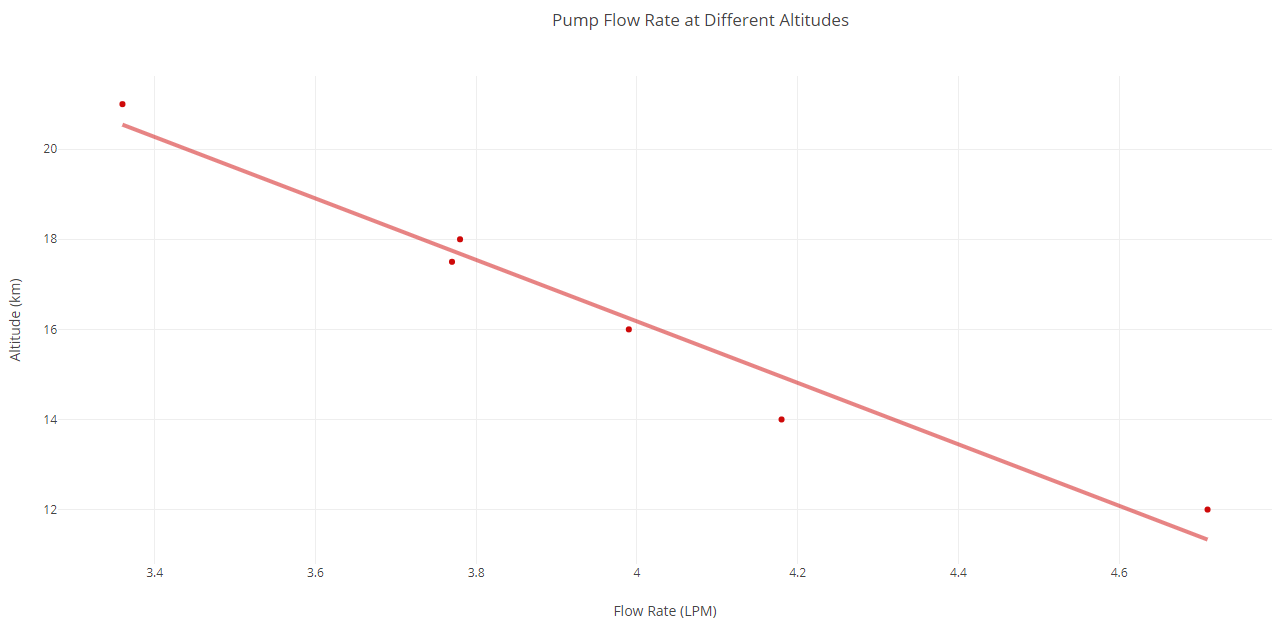
\includegraphics[width=11cm]{5-experiment-verification-and-testing/img/pump-flow-rate-new.png}
    \end{align*}
    \caption {Obtained Pump Performance at Low Pressure.} \label{fig:pump-performance-lowpressue}
\end{figure}

\subsubsection{Test 30: Sampling Bag Bursting}
\label{sec:test30result}

A sampling bag was placed in a small vacuum chamber connected to the pump and the pump was run for 3 minutes with a full bag to see how the bag reacted. 

It was found that there are two potential failure modes. The first is a slow leakage caused by damage to the bag seal and the second is  a rapid failure of the bag seal leading to total loss of the sample.

It can be concluded that, as long as the bags are well secured to the valves at the bottom and through the metal ring at the top, bag bursting during flight would not cause damage to any other components on board. Even during the more energetic burst that occurs from continuous pumping the bag remained fixed to the valve connection and experienced no fragmentation. The consequences of a single bag burst would be limited to loss of data and a disturbance to audio frequencies. 

\subsubsection{Test 29: Pump Current under Low Pressure}
\label{sec:test29result}

In general it was found that decreasing the pressure, or increasing the altitude, lead to a decrease in pump current draw. The full results can be seen in Table \ref{tab:pumpcurrentpressure}. 

\begin{table}[H]
\centering

\begin{tabular}{|l|l|l|l|}
\hline
\textbf{Altitude (km)} & \textbf{Pressure (hPa)} & \textbf{Into Bag Current (mA)} & \textbf{Into Seal Current (mA)} \\ \hline
20 & 57 & 140 & 138 \\ \hline
18 & 68 & 150 & 141 \\ \hline
16 & 100 & 161 & 146 \\ \hline
12 & 190 & 185 & 175 \\ \hline
9 & 300 & - & 200 \\ \hline
6 & 500 & - & 242 \\ \hline
0 & 1013 & - & 218 \\ \hline
\end{tabular}
\caption{Table Showing How the Current Draw of the Pump Changed With Outside Air Pressure for Two Different Conditions. The First Pumping Into a Sampling Bag and the Second Pumping Into a Sealed Tube.}
\label{tab:pumpcurrentpressure}
\end{table}

From the table it can be seen that the current draw is higher during the bag filling than during the sealed case. As the experiment will sample between 11 km and 24 km it can be concluded that the highest current draw will occur during the 11 km altitude sample and can be expected to be around 200 mA. 

\subsubsection{Test 17: Sampling bags' holding times and samples'}
\label{sec:test17result}

The main objective of this test was to flush eight 1 L sampling bags with nitrogen, the same way it will be done for the flight. After the flushing was done, filled them with a dry gas and placed them outside for 6, 14, 24 and 48 hours. Then analyzed two sampling bags after each time duration and saw if the concentration of gases inside has changed. 

The test was done twice as the first test did not give conclusive results.

The general outcome of this test the first time was that the team realized that the flushing of the sampling bags is a very delicate process. This test was also useful to decide that the flushing of the sampling bags should be done with dry gas instead of nitrogen in order to minimize the effects of the nitrogen diluting in the samples. 

This test had to and was repeated, using the set-up described in Section 4, with some differences. This time 3L bags were flushed with dry gas and left outside for 15, 24, 48 hours. After the flushing was done, two bags for each time were filled with 0.5 L and 1L of dry gas and left outside. Then they were analyzed and checked if the sample concentrations were the same or close enough with the reference values of the filled dry gas.

The obtained results are shown in Figure \ref{fig:test17-resultsSEP}. The blue points represent the sampling bags with the 0.5L sample, while the red points show the sampling bags with the 1L sample. Sampling Bag No1 with the sampling bag No4 were analyzed after 15 hours. The pair of sampling bags No2 and No5 were analyzed after 24 hours and the last pair of sampling bags, No4 and No6 after 48 hours.  

\begin{figure}[H]
    \begin{align*}
        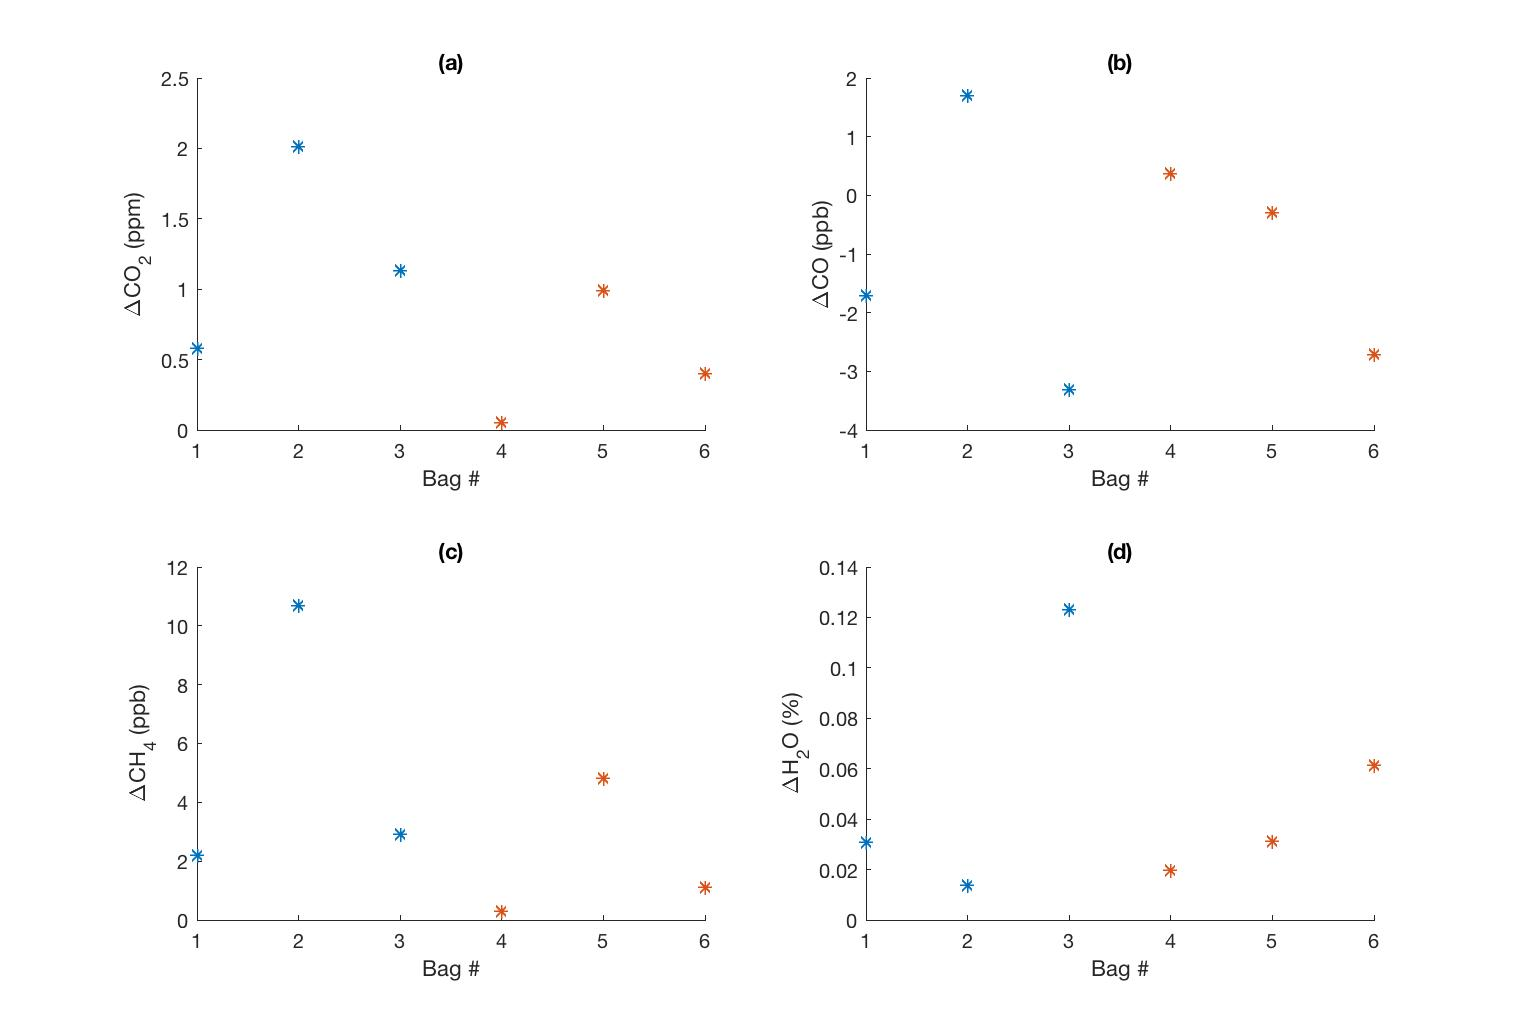
\includegraphics[width=1\linewidth]{5-experiment-verification-and-testing/img/test17resultsSEP.jpg}
    \end{align*}
    \caption {Obtained Variation in Concentration for (a) $CO_2$ in ppm, (b) $CO$ in ppb, (c) $CH_4$ in ppb and (d) $H_2O$ in $\%$.} \label{fig:test17-resultsSEP}
\end{figure}

The results were very good in general with the $CO_2$ concentration differences not higher than 2 ppm. The bags with the 0.5L sample gave bigger $CO_2$ concentration differences and higher humidity for all the tested times. For the bags that analyzed after 48 hours, the humidity was two times higher for the 0.5L sample compared to the 1L sample. If water goes through the walls of the bags at the same rate for both bags then it is normal that sampling bags with larger amounts of sampled air have lower humidity concentrations. Therefore, for better results, the air left in the sampling bags at sea level pressure must be the maximum possible.


\textbf{Efficiency of the flushing procedure.}

While testing the holding times of the sampling bags, some other relevant tests were performed. A sampling bag was flushed the way it will be flushed before flight, and then analyzed immediately. The Picarro readings were very close with the reference values, which means that the flushing procedure is sufficient. From the results obtained when flushing in May, it was also decided to use dry gas for flushing and not nitrogen which has now been confirmed to work better. \\

The humidity levels inside the AAC system were also tested and found to be acceptable. 

\textbf{Flushing over night.}

In addition to the tests performed for the holding times, it was also tested if flushing a sampling bag the night before and sampling it the next day was affecting the samples. A sampling bag was flushed following the same procedure as before and left sealed over night. The next day it was sampled and left outside for almost four hours. Then it was analyzed and the results were compared with a sampling bag that was being flushed and then immediately sampled. The results were good enough with $CO_2$ concentrations being higher in the sampling bag which was flushed the night before. A reasonable result since the $CO_2$ concentration inside a room is higher than outside. Therefore, the team has decided that the flushing of the bags shall be done as late as possible moment before the flight. 

 

% Flushing with nitrogen may alter the results. 

\subsubsection{Test 4: Low Pressure}\label{lowpressure}

\textbf{Styrofoam}

The same vacuum chamber was used as in Tests 18 and 29. The Styrofoam was measured on each side before it was placed in the chamber. It was then taken down to 5 hPa and held there for 75 minutes. It was then removed and the sides were measured again. It was found that there was no significant change in dimensions. The results can be seen in Table \ref{tab:styrofoam-test-result-2}.

\begin{table}[H]
\begin{tabular}{|l|l|l|}
\hline
Side & Before (cm) & After (cm) \\ \hline
A & 9.610 & 9.580 \\ \hline
B & 9.555 & 9.550 \\ \hline
C & 9.560 & 9.565 \\ \hline
D & 9.615 & 9.610 \\ \hline
E & 9.615 & 9.615 \\ \hline
F & 9.555 & 9.550 \\ \hline
G & 9.605 & 9.605 \\ \hline
H & 5.020 & 5.020 \\ \hline
I & 5.025 & 5.025 \\ \hline
J & 5.015 & 5.015 \\ \hline
K & 5.020 & 5.025 \\ \hline
\end{tabular}
\caption{Styrofoam Size Before and After Vacuum.}
\label{tab:styrofoam-test-result}
\end{table}

\textbf{Airflow}

After the first airflow in vacuum test failed due to datalogging errors the airflow test was repeated. In this repeated test all of the Brain was placed into the vacuum chamber and one bag attached. It was not possible to attach more than one bag due to space restrictions. 

The flow rate seemed to be too low for the rate the bag was inflating in the chamber. It was concluded that the airflow rate displayed is the equivalent airflow at sea level. 

\textbf{Software}

With the same set-up as the airflow low pressure testing the software was tested to verify if it was operating as intended and that the conditions for stopping sampling were working.

The software was found to be operating as intended and the stoppers were working. 

\textbf{Temperatures}

As it is not possible to complete a thermal vacuum test in addition to the thermal testing  temperatures were also monitored inside the vacuum chamber.

The temperature of the CAC flushing valve, pressure sensor, PCB, Pump and Manifold was also monitored with continuous use. After one hour and 48 minutes during the same test as the valve temperature the CAC flushing valve was found to reach 68$\degree{C}$ and the pressure sensor was found to reach 39$\degree{C}$. After one hour and 24 minutes during the flow rate monitoring test where the sensors, pump, and one manifold valve were on continuously the PCB temperature sensor was at 43$\degree{C}$, the pump at 42$\degree{C}$ and the manifold at 33$\degree{C}$. As the pump will never be on for more than a few minutes at a time there is not any concern that this temperature will ever be reached during flight.

\subsubsection{Test 20: Switching Circuit Testing and Verification}

The switching circuit has been continuously tested from breadboard to PCB and verified to work at each different step. All valves, heaters and pump can be controlled both manually and automatically by the Arduino. For further details on this test see Appendix \ref{sec:test33result}.

\subsubsection{Test 32: Software Failure}

it was found that losing the SD card does not interrupt ground station data, it just means no data will be written to the SD card. However, if you reconnect the SD after removing it will not connect back to the SD card and it as if the SD card has been permanently lost.\par

The second failure test is how the software handles unexpected reset. The most concerning problem is which bag that will be sampled after the reset. It has been tested that the software could read the current sampling status from SD card and continue where it left off. 

\subsubsection{Test 31: Unit Test}
Unit test was used to test several software non-hardware dependent functionality e.g. translating telecommand, storing measurements data to buffer. The functions were tested for several expected cases and a few bugs were discovered and fixed.

\subsubsection{Test 10: Software and Electronics Operation}
OBS transmits data to ground station continuously. If connection is lost and later re-established the ground station will continue to receive data from the onboard computer. To send a telecommand after a drop in connection requires a restart to the TCP connection. 

\subsubsection{Test 14: Ground Station-OBC Parameters Reprogram Test}
After the scheduler, a command to change the sampling parameters, is implemented, the scheduler was tested and can change the sampling schedule from ascent to descent. The previous parameters were $56.8$ and $36.8$. They were successfully changed to $30$ and $70$. However, the user needs to be careful and has to do the correct calculation for the new parameters.

\subsubsection{Test 24: Software and Electronics Integration}
The different type of sensors were integrated one at time with the Arduino. The result was all the sensors working without interfering with each other.



\subsubsection{Test 5: Thermal Test} \label{Test-5}
From the thermal test completed at FMI it can be concluded that the regulation for keeping the critical components above lower operating temperature is working. As seen in Figure \ref{fig:test-5-thermal-chap5} both the pump (purple) and the manifold (blue) have their heaters turning on when the temperature gets to the lower threshold. The dotted vertical line is where the temperature sensors got error in communication.

\begin{figure}[H]
    \centering
    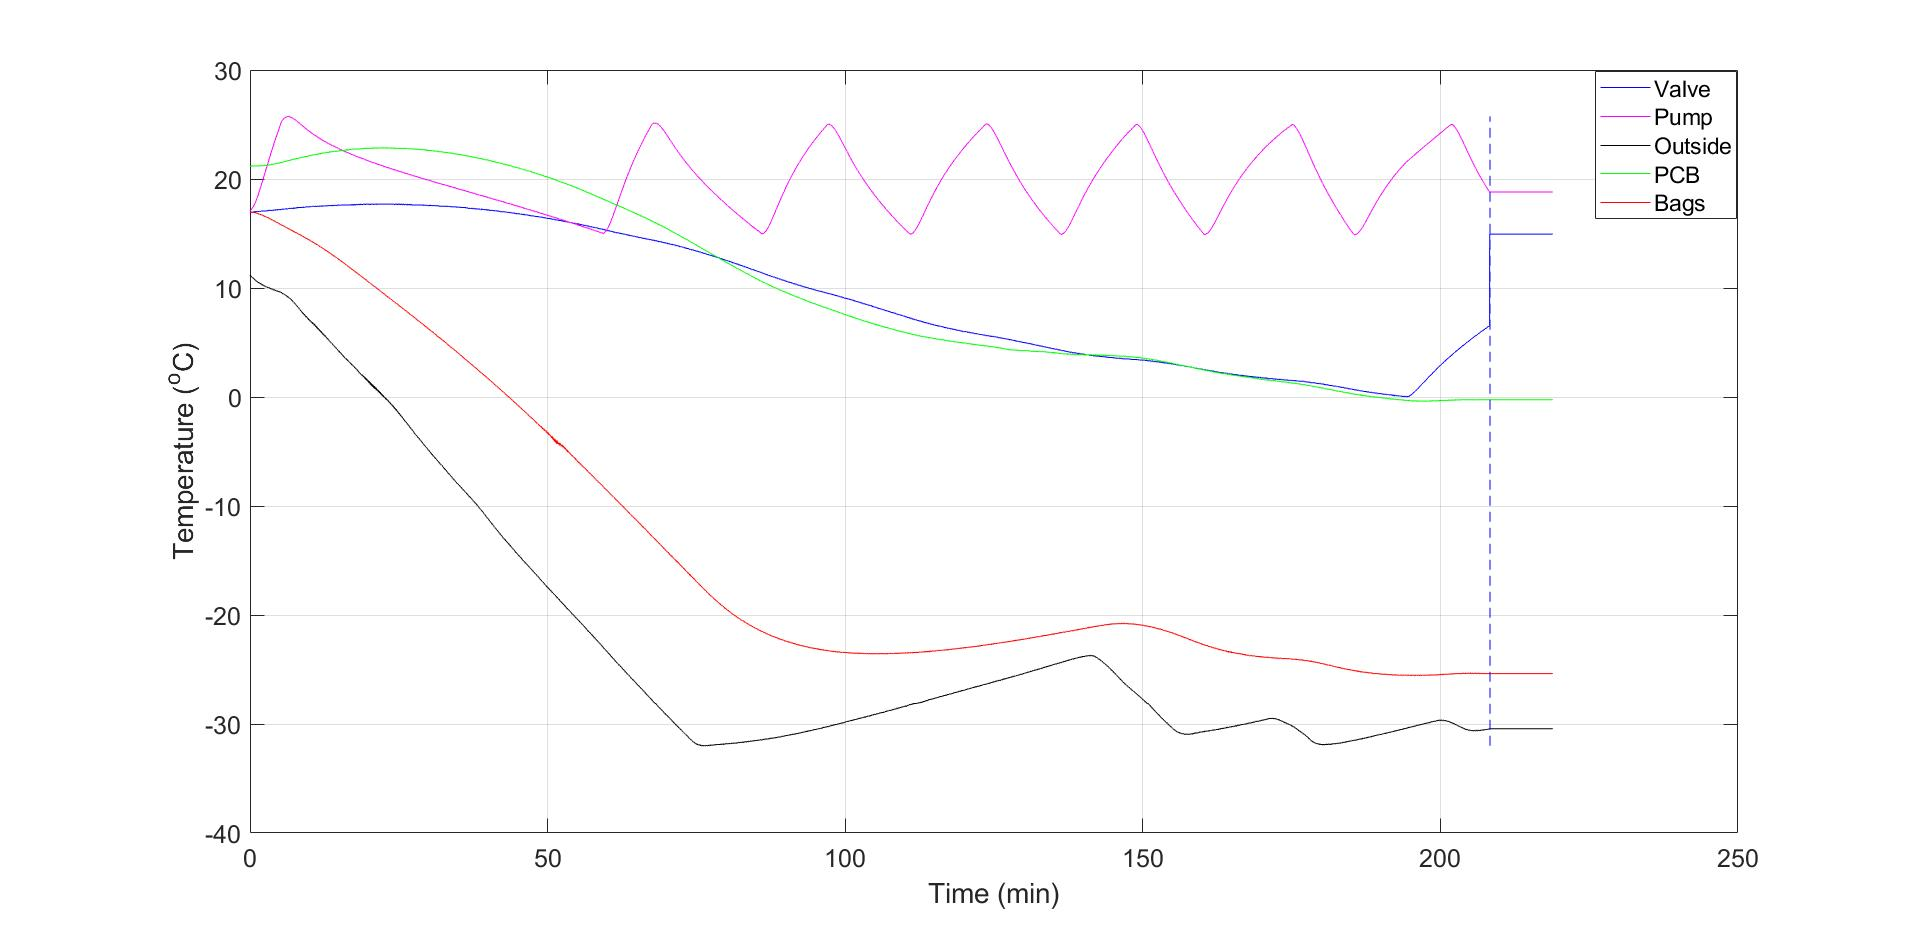
\includegraphics[width=\linewidth]{5-experiment-verification-and-testing/img/Thermal-Test-3.jpg}
    \caption{Thermal Chamber Test.}
    \label{fig:test-5-thermal-chap5}
\end{figure}

Further testing in the university freezer down to $-20\degree{C}$ was also undertaken for 6 and 8 hours with no problems seen. Final testing will take place at Esrange on the 5th October as a final verification.

\subsubsection{Test 27: Shock test}
The entire pneumatic system and electrical system was mounted in the AAC box along with the walls and Styrofoam attached. It was then dropped from a height of approximately one meter three times. Nothing came loose or was damaged after this drop test. All electronics were verified to still work.

\subsubsection{Test 9: Vibration test}
The entire experiment was placed in the tailgate of a car, while the test was carried out on a 18 km long rough terrain. An emergency brake was also implemented during the test. The experiment's functionality and structural integrity were capable of handling the vibrations and the stopping force.
No damages or issues were detected after this test. 

\subsubsection{Test 25: Structure test}
A team member was placed on top of each box's structure. Both the CAC and AAC box was able to fully support the member's weight without showing any instability or deflections. No damages or issues were detected after this test. 

\subsubsection{Test 33: Electrical Component Testing}
\label{sec:Test33Test-Electronical-Component-Testing}
The components were tested separately, one by one to double check and determine their power consumption and their functionality. Some tests were also run to determine specific resistances on voltage bridges and pull down resistors for LEDs running at different voltages. These tests gave further insight to the PCB design and the power design. The test results were according to expectations and the design and assembly could continue as planned. There were also some test run for the PCB, which showed that some connections were not done in the way that was planned due to design issues. Theses were solved by adding wires to the PCB instead of redesigning the PCB and order a new one due to time and budget limitations. For further details on these tests see Section \ref{sec:test33result}.

\subsubsection{Test 12: Removal test}
For a non team member to perform the removal of the CAC box based on the given instructions, it took that person 6 min and 25 sec. This time is expected to be lower for the recovery team as the items to be unscrewed were not yet clearly marked. One problem that occurred during this test was that the person had problems to distinguishing the CAC from the AAC box. To resolve this the boxes now have clear labels on them.

\subsubsection{Test 2: Data collection test}
The full software was run in auto mode to check everything operated as expected over a full test flight. At the end of the simulated flight the experiment was to shutdown automatically. This was tested both on the bench and in the vacuum chamber. In the vacuum chamber tests, see Section \ref{lowpressure}, the bench test, see Appendix \ref{benchtest} and the thermal test, see Appendix \ref{thermaltestresults} data collection was also monitored. It was found that the physical samples were being collected properly and all the sensors were returning expected data.


\subsubsection{Test 7: Bench test}\label{benchtest}
The experiment was run for 5 hours simulating 1 hour on ground, 1.5 hours in ascent, 2 hours in float and 0.5 hours in descent. The experiment was found to be operating as intended at all points. Additionally the temperature sensors have been tested at ambient conditions for over 6 hours and the pressure sensors for over 8 hours. No problems were found with the temperature sensors or pressure sensors on the bench. 

 

\subsubsection{Test 16: Sampling test}
The system was tested while already mounted as this test was pushed back due to the late arrival of the static pressure sensor.

The Arduino successfully controlled all valves and the pump and through the static pressure and airflow sensor readings alone it could be confirmed if a bag was sampling.

